\documentclass{article}
\usepackage[paperwidth=5.5cm,paperheight=5.3cm,left=0cm,right=0cm,bottom=0cm,top=0.25cm]{geometry}
\usepackage{tikz}
\definecolor{fom}{RGB}{0,153,139}
 
\newcommand{\dat}{0.7} % 0.67
\usepackage{animate}
 
\begin{document}
 
\begin{animateinline}[poster=last, controls, palindrome]{10}
\multiframe{70}{Ry=0.1+0.01}{
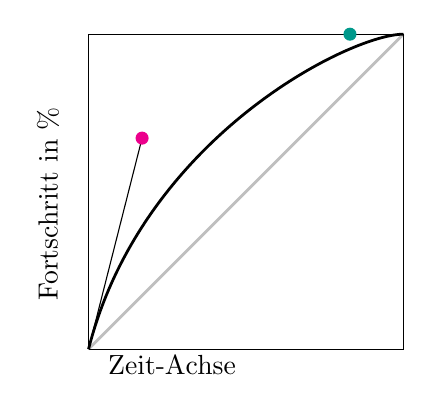
\begin{tikzpicture}[x=4cm,y=4cm]
\draw[line width=1pt,lightgray] (0,0) -- (1,1);
\draw (0,0) -- (1,0) -- (1,1) -- (0,1) -- (0,0); 
\draw (0,0) -- (0.17,0.67); 
\draw (1,1) -- (0.83,\Ry); 
 
\draw [magenta,fill=magenta](0.17,0.67) circle (.5ex); 
\draw [fom,fill=fom](0.83,\Ry) circle (.5ex); 
 
\draw[line width=1pt] (0,0) .. controls (0.17,0.67) and (0.83,\Ry) .. (1,1);
 
\node[label={[label distance=0.0cm,text depth=-1ex,rotate=90]left:Fortschritt in \%}] at (-0.1,.8) {};
\node[label={[label distance=0.0cm,text depth=-1ex]right:Zeit-Achse}] at (0,-0.05) {};
\end{tikzpicture}}
\end{animateinline}
 
\end{document}